
\begin{frame}{Nitrogen Vacancy Centre in diamond (NV center)} %{{{1
  \begin{center}
    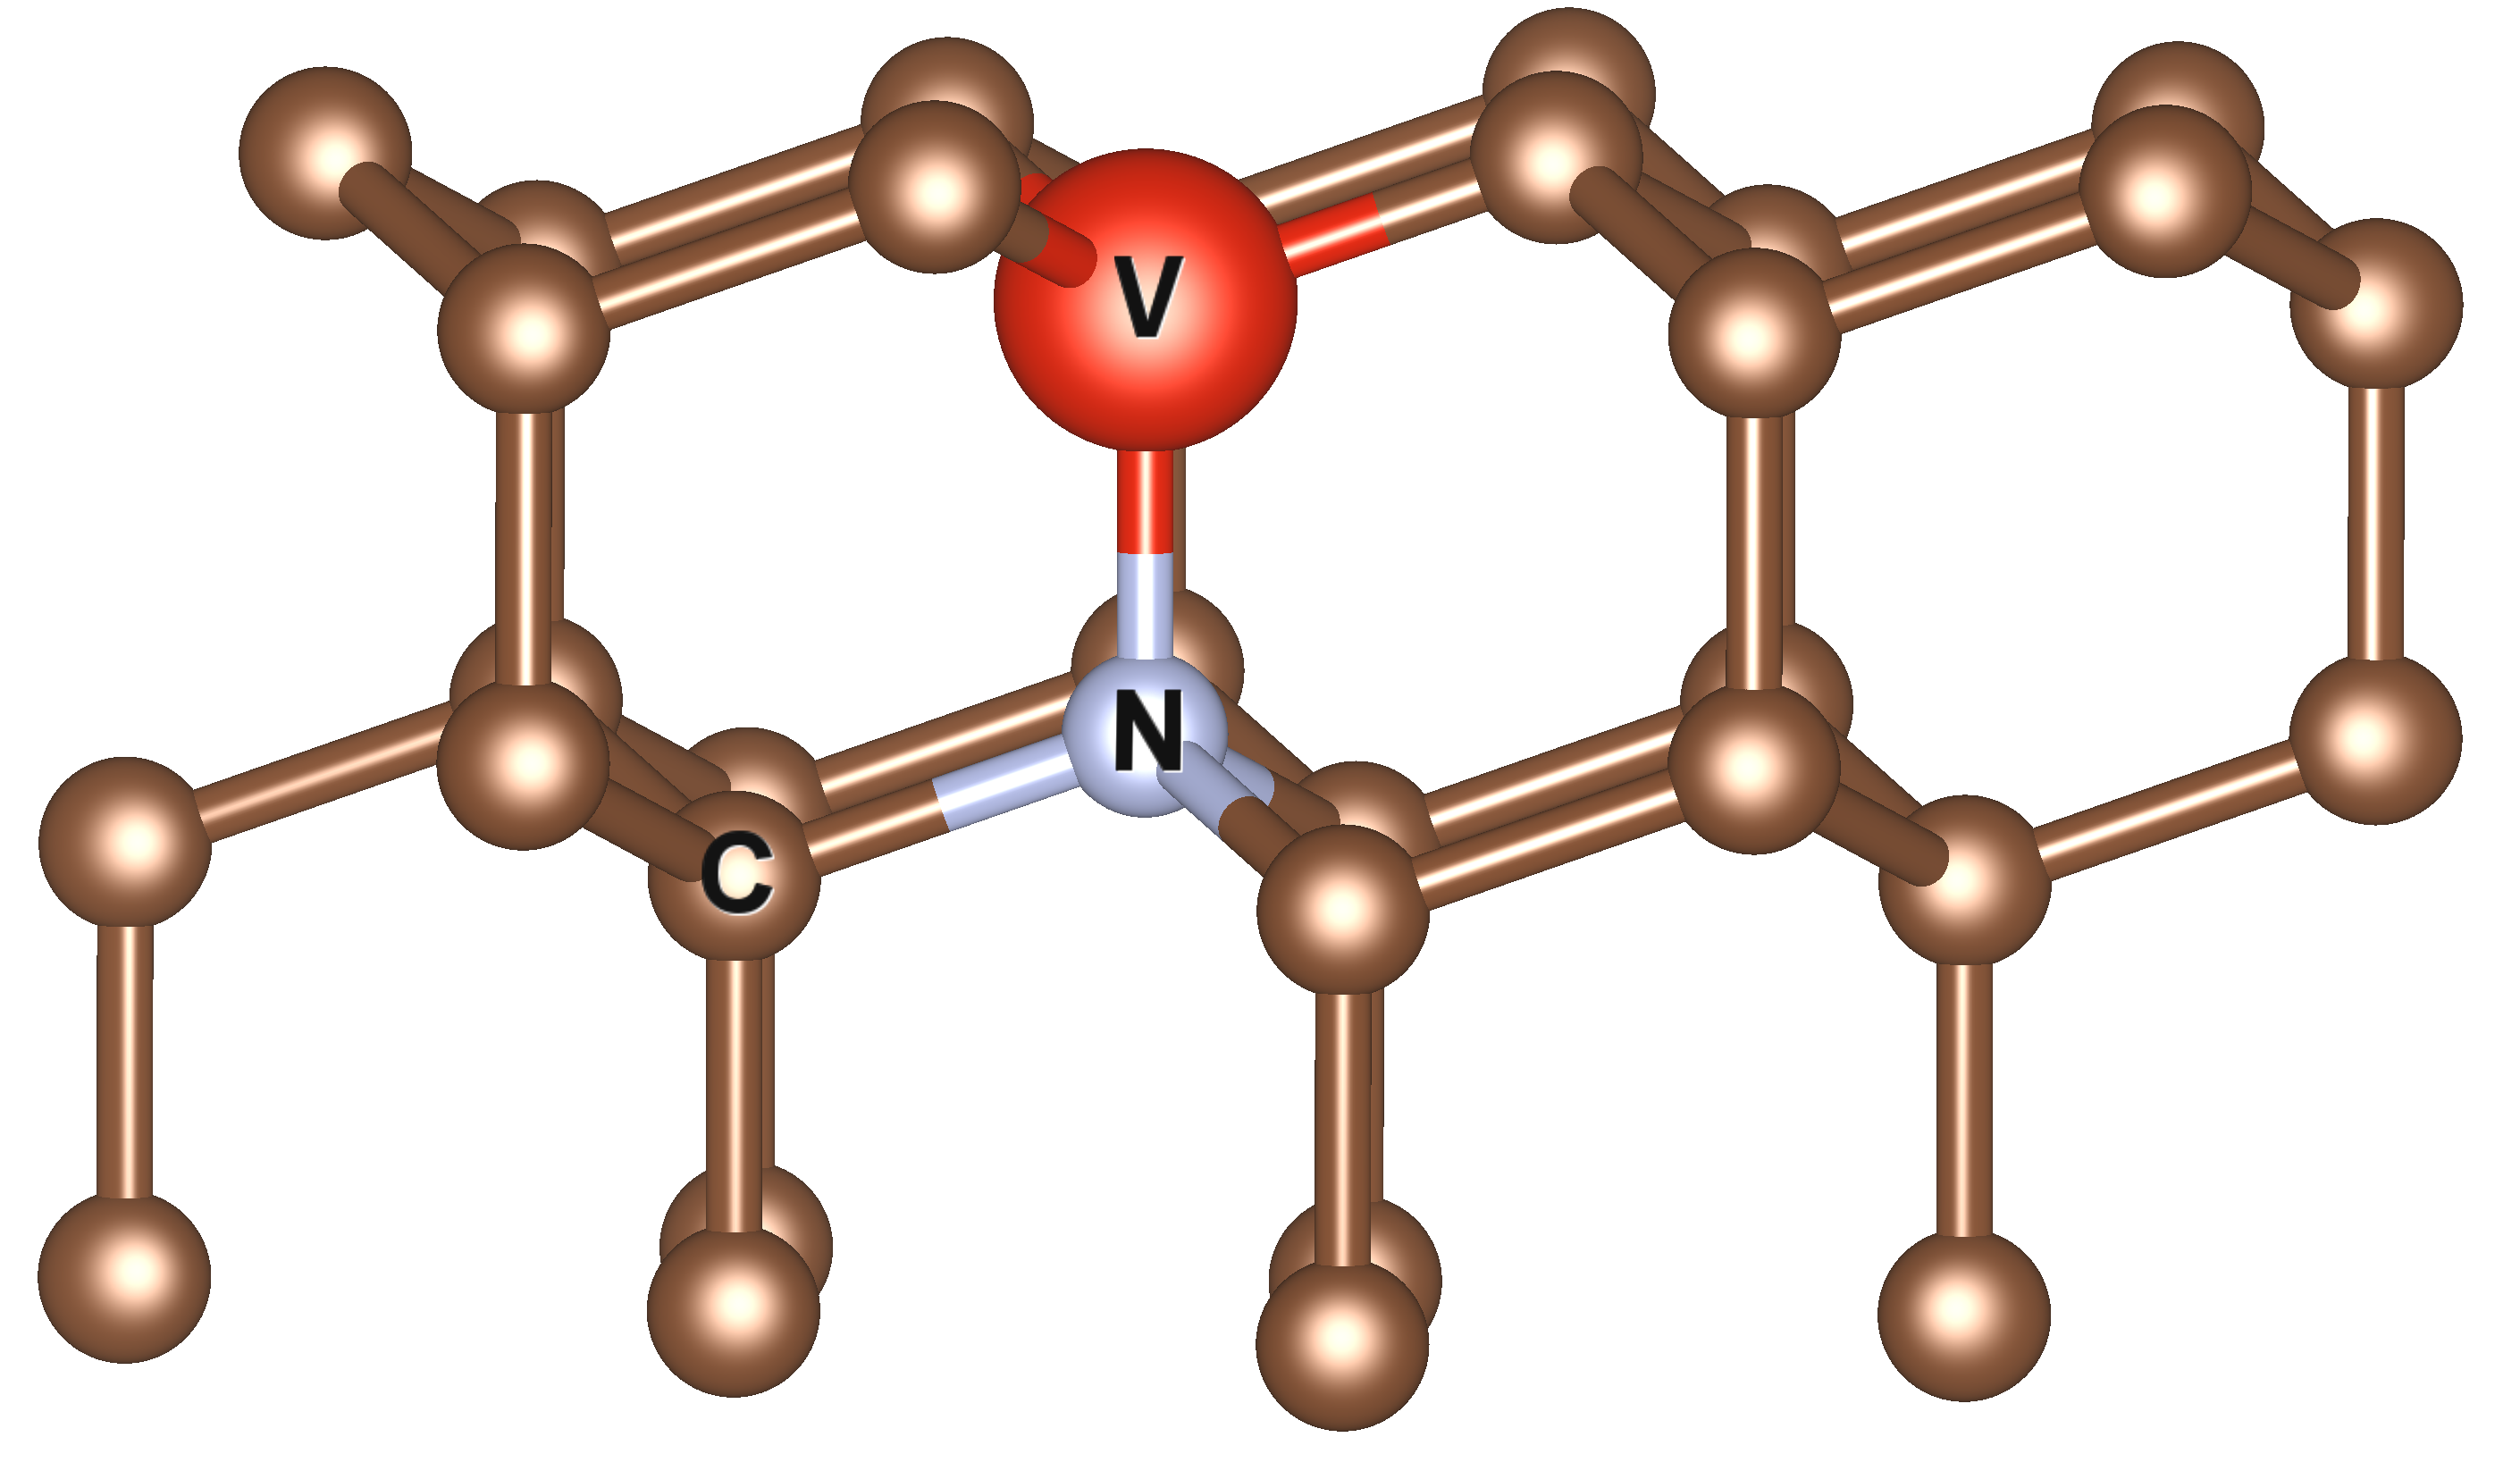
\includegraphics[width=0.9\textwidth]{images/POSCAR_16_view.png}
  \end{center}

  \note{

    So let us just begin by firstly introducing the main actor in this story.
    This is the Nitrogen vacancy impurity center in diamond, as most of you may
    already know.  The big red region is a vacant carbon site and next to it
    lies a nitrogen atom.

    This kind of defects has been researched now for almost 50 years.  However
    it was not until the late nineties when single negatively charged NV
    centres where found. This enabled the demonstration of photo stable single
    photon emitters, which is of course of huge importance for quantum optics.

    The most notable and studied of the NV centers is the negatively charged
    one.

  }

\end{frame}

